\documentclass[12pt]{scrartcl}

 

\usepackage{float}

\usepackage[utf8]{inputenc}

\usepackage[T1]{fontenc}

\usepackage{lmodern}

\usepackage[ngerman]{babel}

\usepackage{amsmath}

\usepackage{graphicx}


 

\title{Versuch MI1\\ Mikrowellen}

\author{Frederik Strothmann, Henrik Jürgens}

\date{\today}


\begin{document}


 %deckblatt erstellen

\maketitle
\tableofcontents
\newpage

%einleitung zu dem experiment

\section{Einleitung}

Ein System aus Mikrowellensender und verschiedenen Empfängern ermöglicht Untersuchungen verschiedener physikalischer Effekte an Mikrowellen. So sollen in diesem Versuch stehende Wellen vermessen werden, außerdem wird die Wirkung einer Wachs-Sammellinse oder eines Polfilters (parallele Metallstäbe) untersucht sowie die Reflexion
an einer Wachsplatte (Brewster-Winkel), die Totalreflexion zwischen einer Wachs-Luft-
Wachs-Schicht und die Drehung der Polarisationsebene durch
”optisch aktive“ Substanzen.
(Spiralfedern in einem Styroporträger)
%versuchsaufbau mit skizze

\section{Versuchsaufbau}

%wenn du tabellen einfügst dann schreib bitte anstatt [htpb] [H]. zusammen mit \usepackage{float} verrutscht dann garnichts mehr
\section{Versuchsdurchführung}


\subsection{Praktische Durchführung}
\textbf{Allgemeine Hinweise:}\\
Die Mikrowellensender werden mit einer Gleichspannung von ca. 10 bis 12 V versorgt.
\begin{enumerate}
\item Zunächst stellen wir den Sender und eine Metallplatte im Abstand von ca. 30 - 40 cm gegenüber auf und zwischen beide die Diode. Dadurch bildet sich eine stehende Welle, sodass wir durch Verschieben der Metallplatte die Wellenlänge messen können.
\item
Wir messen die Intensitätsverteilung senkrecht zur Strahlrichtung mit dem Hornempfänger, wobei uns eine Wachslinse zur Verfügung stand:
\begin{enumerate}
\item ohne Linse (Abstand Sender-Empfänger ca. 1,5 m)
\item mit Linse (Abstand Sender-Linse 0,5 m, Linse-Empfänger 1 m)
\end{enumerate}

\item Die Totalreflexion der Mikrowellen soll anhand des folgenden Versuchs untersucht werden:

%hier die Abbildung aus der Versuchsanleitung einfügen, footnote muss noch geschrieben werden.
\begin{figure}[H] 
  \centering
    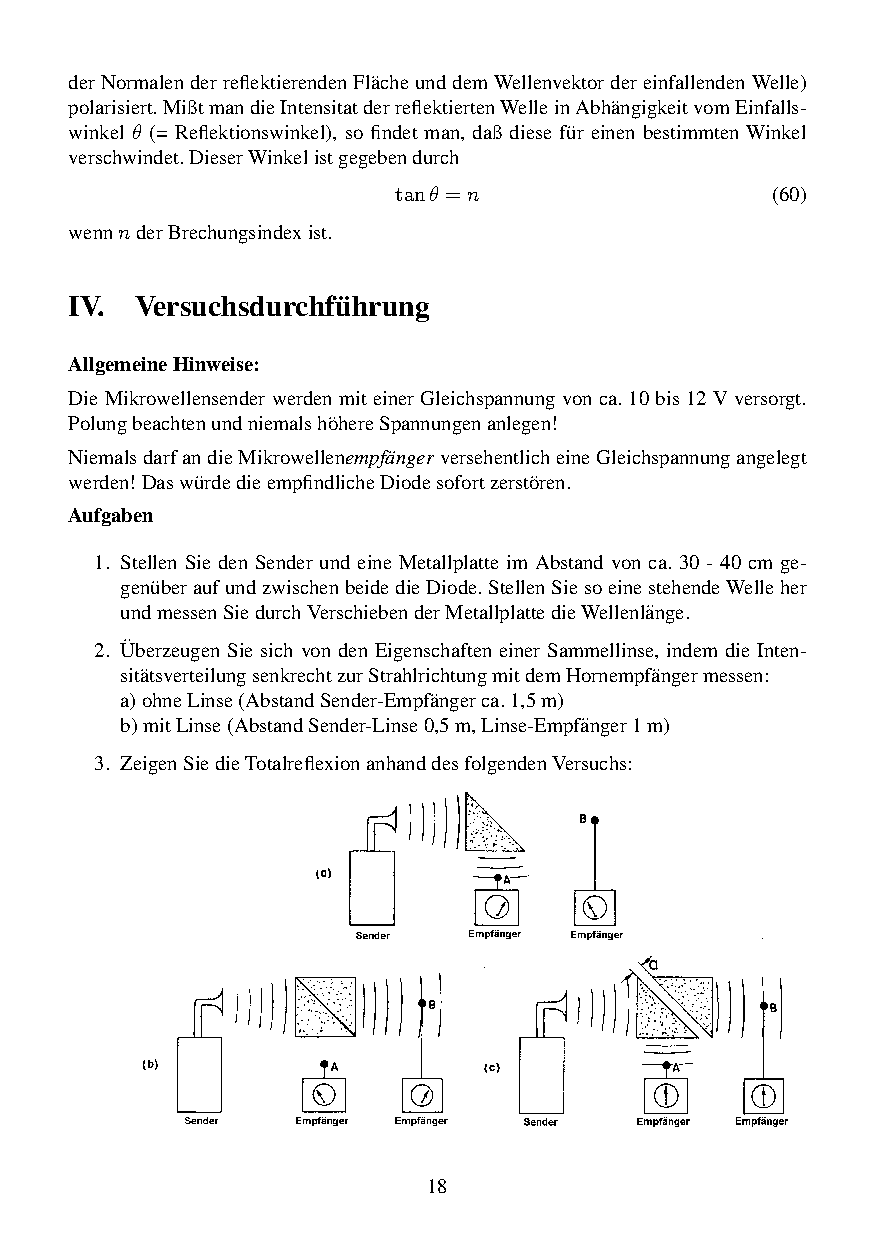
\includegraphics[trim = 0mm 15mm 0mm 132mm, clip, scale = 1]{totalreflexion.pdf}
  	\caption[Abbildung der beiden Schaltungen, für die Bestimmung des Wiederstandes]{Abbildung der beiden Schaltungen, für die Bestimmung des Wiederstandes\footnotemark}
  \label{fig:abb_versuch_3}
\end{figure}
\footnotetext{Abbildung entnommen von http://www.atlas.uni-wuppertal.de/~kind/MI1.pdf Seite 18 am 16.08.2014}

Die Wachsprismen werden ( n = 1,5 ) wie in Abbildung (c) gezeichnet im Abstand a gegenüber gestellt. Wir messen nun die Intensität des Empfängers in Abhängigkeit des Abstandes a.
%Versuchen Sie, die Erscheinung zu erklären.
\item In dieser Aufgabe stellen wir Sender und Empfänger  so gegenüber, dass die Polarisationsrichtungen (Richtungen, in denen der E-Vektor schwingt) der beiden parallel sind. Im Folgenden drehen wir den Empfänger um die Verbindungslinie von Sender und Empfänger und messen die Intensität in Abhängigkeit des Drehwinkels.

\item Sender und Empfänger nun um 90$^{\circ}$ gedreht gegenüber gestellt. Ein Gitter wird so zwischen Sender und Empfänger gehalten, dass die Stäbe mit dem E-Vektor einen Winkel von 45$^{\circ}$ bilden. Wir messen dazu die Intensität mit und ohne Gitter.

\item Abhängig vom Einfallswinkel messen wir die Intensität der von einer Wachsplatte reflektierten Wellen, die parallel zur Einfallsebene polarisiert sind. Daraus bestimmen wir den Brechungsindex.

\item Wir wollen die Drehung der Polarisationsebene durch ”optisch aktive“ Substanzen untersuchen. Es gibt dazu optisch aktive mit Rechtsschraubenfedern besetzte Styroporplatten. Die Platten sind durch eine Markierung (R) an der Seite der Styroporplatten gekennzeichnet.
\end{enumerate}

\subsection{Theoretische Durchführung}

\begin{enumerate}
\item
\item
\item
\item
\item
\item
\item
\end{enumerate}

\section{Messergebnisse}

\subsection{Aufgabe 1}
\begin{table}[H]
\caption{Abstandsmessungen der ersten Aufgabe, der Feherl beträgt bei allen Werten $(\pm 0,005)$}
\begin{tabular}{|r|}
\hline
\multicolumn{1}{|l|}{d/m} \\ \hline
0,36 \\ \hline
0,3735 \\ \hline
0,387 \\ \hline
\end{tabular}
\label{tab:a_1}
\end{table}

\subsection{Aufgabe 2}
\begin{table}[H]
\caption{Daten der Messung ohne Linse. Für den Fehler des Strom wurde ein Wert von $(\pm 1)$ und für die Positon wurde ein Fehler von $(\pm 0,1)$ angenommen.}
\begin{tabular}{|r|r|}
\hline
\multicolumn{1}{|l|}{Strom/$\mu$A} & \multicolumn{1}{l|}{p/cm} \\ \hline
67 & 0 \\ \hline
68 & -1 \\ \hline
65 & -2 \\ \hline
63 & -3 \\ \hline
61 & -4 \\ \hline
61 & -5 \\ \hline
71 & 1 \\ \hline
70 & 2 \\ \hline
69 & 3 \\ \hline
68 & 4 \\ \hline
68 & 5 \\ \hline
\end{tabular}
\label{tab:a_2_o}
\end{table}

\begin{table}[H]
\caption{Daten der Messung mit Linse. Für den Fehler des Strom wurde ein Wert von $(\pm 1)$ und für die Positon wurde ein Fehler von $(\pm 0,1)$ angenommen.}
\begin{tabular}{|r|r|}
\hline
\multicolumn{1}{|l|}{Strom/$\mu$A} & \multicolumn{1}{l|}{p/cm} \\ \hline
53 & 0 \\ \hline
52 & -1 \\ \hline
51 & -2 \\ \hline
50 & -3 \\ \hline
47 & -4 \\ \hline
44 & -5 \\ \hline
50 & 1 \\ \hline
48 & 2 \\ \hline
45 & 3 \\ \hline
42 & 4 \\ \hline
40 & 5 \\ \hline
\end{tabular}
\label{tab:a_2_m}
\end{table}

\subsection{Aufgabe 3}

\begin{table}[H]
\caption{Daten der Messung mit nur einem Block.}
\begin{tabular}{|l|l|}
\hline
Strom\_a/ $\mu$A & Strom\_b / $\mu$A \\ \hline
4 $(\pm1)$ & 140 $(\pm 5)$ \\ \hline
\end{tabular}
\label{tab:a_3_e}
\end{table}

\begin{table}[H]
\caption{Daten der Messung mit beiden Blöcken zusammen, der Fehler ist bei beiden Werten $(\pm 1)$}
\begin{tabular}{|l|l|}
\hline
Strom\_a/$\mu$A & Strom\_b/$\mu$A \\ \hline
\multicolumn{1}{|r|}{81} & \multicolumn{1}{r|}{0,4} \\ \hline
\end{tabular}
\label{tab:a_3_z}
\end{table}

\begin{table}[H]
\caption{Daten der Messung für das auseinanderschieben der Blocke.  Der Fehler für a wurde mit $(\pm 0,1)$ und für Strom\_a $(\pm 1)$ angenommen.}
\begin{tabular}{|r|r|r|r|}
\hline
\multicolumn{1}{|l|}{a/cm} & \multicolumn{1}{l|}{Strom\_a/$\mu$A} & \multicolumn{1}{l|}{Strom\_b/$\mu$A} & \multicolumn{1}{l|}{Fehler/$\mu$A} \\ \hline
0,5 & 49 & 65 & 1 \\ \hline
1 & 29 & 90 & 2 \\ \hline
1,5 & 22 & 129 & 2 \\ \hline
2 & 19 & 147 & 4 \\ \hline
3 & 18 & 165 & 2 \\ \hline
\end{tabular}
\label{tab:a_3_m}
\end{table}

\subsection{Aufgabe 4}

\begin{table}[H]
\caption{Daten der Messung für das auseinander Schieben der Blöcke. Der Fehler für a wurde mit $(\pm 0,1)$ und für Strom\_a mit $(\pm 1)$ angenommen.}
\begin{tabular}{|r|r|}
\hline
\multicolumn{1}{|l|}{Winkel/grad} & \multicolumn{1}{l|}{Strom/$\mu$A} \\ \hline
0 & 191 \\ \hline
5 & 188 \\ \hline
10 & 181 \\ \hline
15 & 177 \\ \hline
20 & 174 \\ \hline
25 & 162 \\ \hline
30 & 153 \\ \hline
35 & 137 \\ \hline
40 & 119 \\ \hline
45 & 108 \\ \hline
50 & 91 \\ \hline
55 & 77 \\ \hline
60 & 63 \\ \hline
65 & 47 \\ \hline
70 & 32 \\ \hline
75 & 19 \\ \hline
80 & 9 \\ \hline
85 & 3 \\ \hline
90 & 2 \\ \hline
\end{tabular}
\label{tab:a_4}
\end{table}


\subsection{Aufgabe 5}

\begin{table}[H]
\caption{Messdaten ohne Gitter.}
\begin{tabular}{|l|l|}
\hline
Strom/$\mu$A & Fehler/$\mu$A \\ \hline
\multicolumn{1}{|r|}{1} & \multicolumn{1}{r|}{1} \\ \hline
\end{tabular}
\label{tab:a_5_o}
\end{table}

\begin{table}[H]
\caption{Messdaten mit Gitter.}
\begin{tabular}{|l|l|}
\hline
Strom/A & Fehler/A \\ \hline
\multicolumn{1}{|r|}{86} & \multicolumn{1}{r|}{1} \\ \hline
\end{tabular}
\label{tab:a_5_m}
\end{table}

\subsection{Aufgabe 6}

\begin{table}[H]
\caption{Messdaten für die bestimmung des Brewsterwinkel. Der Fehler für den Winkel wurde mit $(\pm 2)$ und der Strom mit $(\pm 0,05)$ angenommen.}
\begin{tabular}{|r|r|}
\hline
\multicolumn{1}{|l|}{Winkel/grad} & \multicolumn{1}{l|}{Strom/$\mu$A} \\ \hline
10 & 0,23 \\ \hline
15 & 0,65 \\ \hline
20 & 0,45 \\ \hline
25 & 0,35 \\ \hline
30 & 1,5 \\ \hline
35 & 4 \\ \hline
40 & 6 \\ \hline
45 & 6,5 \\ \hline
50 & 8,3 \\ \hline
55 & 10,2 \\ \hline
60 & 8,8 \\ \hline
65 & 6 \\ \hline
70 & 1,85 \\ \hline
75 & 3,8 \\ \hline
80 & 8,2 \\ \hline
\end{tabular}
\label{tab:a_6}
\end{table}

\subsection{Aufgabe 7}

\begin{table}[H]
\caption{Daten der Messung ohne Substanz.}
\begin{tabular}{|l|l|l|l|}
\hline
Strom/$\mu$A & Fehler/$\mu$A & Winkel/grad & Fehler/grad \\ \hline
\multicolumn{1}{|r|}{0,8} & \multicolumn{1}{r|}{0,05} & \multicolumn{1}{r|}{90} & \multicolumn{1}{r|}{1} \\ \hline
\end{tabular}
\label{tab:a_7_o}
\end{table}

\begin{table}[H]
\caption{Daten der Messung mit Substanz.}
\begin{tabular}{|r|r|r|r|}
\hline
\multicolumn{1}{|l|}{Strom/$\mu$A} & \multicolumn{1}{c|}{Fehler/$\mu$A} & \multicolumn{1}{l|}{Winkel/grad} & \multicolumn{1}{l|}{Fehler/grad} \\ \hline
3,2 & 0,05 & 90 & 1 \\ \hline
0,8 & 0,005 & 97 & 1 \\ \hline
\end{tabular}
\label{tab:a_7_m}
\end{table}





\section{Auswertung}
\subsection{Aufgabe 1}
In der ersten Aufgabe sollte die Wellenlänge des Senders bestimmt werden, dabei wurden drei verschiedene Positionen gemessen siehe Tabelle \ref{tab:a_1} es ergab sich in Mittelwert von:

\begin{align*}
2,7 (\pm 0,2) cm
\end{align*}


Auf dem Sender war ein Wert von 2,8 cm für die Wellenlänge angegeben.

\subsection{Aufgabe 2}
In der zweiten Aufgabe sollte der Effekt einer Sammellinse überprüft werden.
Dafür wurden Sender und Empfänger in einem Abstand von 1,5 Metern zueinander aufgestellt und die Intensität entlang der Orthogonalen vermessen. Dies geschah einmal mit der Sammellinse dazwischen und einmal ohne. Für die Messung ohne Sammellinse ergab sich der folgende Plot (Messwerte aus Tabelle \ref{tab:a_2_o}).

\begin{figure}[H]
\centering
    \includegraphics[scale = 1]{a_2_o.pdf}
  	\caption[Plot der Messung ohne Sammellinse]{Plot der Messung ohne Sammellinse}
  \label{fig:a_2_o}
\end{figure}

Bei der Messung mit Sammellinse ergab sich der folgende Plot (Messwerte aus Tabelle \ref{tab:a_2_m}).


\begin{figure}[H]
\centering
    \includegraphics[scale = 1]{a_2_m.pdf}
  	\caption[Plot der Messung mit Sammellinse]{Plot der Messung mit Sammellinse}
  \label{fig:a_2_m}
\end{figure}



\subsection{Aufgabe 3}
In der dritten Aufgabe sollte die Totalreflexion mit Wachsprismen bestimmt werden.
Dabei ergab  sich bei der Intensitätsmessung mit nur einem Prismen  für Empfänger B ein Wert von 4	$(\pm 1) \mu$A und für Empfänger A ein Wert von 140 $(\pm 5) \mu$A.

Bei der Messung ohne eine Abstand zwischen den Prismen, ergab sich für Empfänger B ein Wert von 0,4 $(\pm 1) \mu$A und für Empfänger A ein Wert von 81 $(\pm 1) \mu$A.

Bei der Vermessung der Intensität in Abhängigkeit des Abstandes der Beiden Platten ergab sich für Empfänger A der folgende Plot (Messwerte aus Tabelle \ref{tab:a_3_m}).

\begin{figure}[H]
\centering
    \includegraphics[scale = 1]{a_3_A.pdf}
  	\caption[Plot der Intensität an Empfänger A, in Abhängigkeit vom Abstand]{Plot der Intensität an Empfänger A, in Abhängigkeit vom Abstand}
  \label{fig:a_3_A}
\end{figure}

Für Empfänger B ergab sich der folgende Plot (Messwerte aus Tabelle \ref{tab:a_3_m} ).

\begin{figure}[H]
\centering
    \includegraphics[scale = 1]{a_3_B.pdf}
  	\caption[Plot der Intensität an Empfänger B, in Abhängigkeit vom Abstand]{Plot der Intensität an Empfänger B, in Abhängigkeit vom Abstand}
  \label{fig:a_3_B}
\end{figure}

Dieser Effekt erklärt sich einerseits durch Streuung an der Grenzschicht und anderseits durch in Schwingung versetzte Atome.

\subsection{Aufgabe 4}
In der vierten Aufgabe sollte die Intensität in Abhängigkeit des Winkels zwischen Sender und Empfänger bestimmt werden. Dabei ergab sich der folgende Plot (Messwerte aus Tabelle \ref{tab:a_4}).

\begin{figure}[H]
\centering
    \includegraphics[scale = 1]{a_4.pdf}
  	\caption[Plot der Intensität in Abhängigkeit des Winkels zwischen Sender und Empfänger]{Plot der Intensität in Abhängigkeit des Winkels zwischen Sender und Empfänger}
  \label{fig:a_4}
\end{figure}

Die Messdaten wurden mit der der Funktion $ f(x) = m \cdot cos(x \cdot n) + b$ gefittet, dabei ergaben sich für die Fitparameter die folgenden Werte, m = 98 $(\pm 1)$, n = 0,0315 $(\pm 0,0005)$ und b = 92 $(\pm 2)$. Das reduzierte Chiquadrat ergab sich mit 1,52196.

\subsection{Aufgabe 5}
In der fünften Aufgabe sollte zwischen die um 90 Grad gegeneinander verdrehten Sender und Empfänger ein Gitter im 45 Grad Winkel zur Polarisationsrichtung gesetzt werden. Dabei ergab sich ein Wert von 1 $(\pm 1) \mu$A ohne Gitter und ein Wert von 86 $(\pm 1) \mu$A mit Gitter.

\subsection{Aufgabe 6}
In der sechsten Aufgabe sollt der Brechungsindex eines Wachsblocks bestimmt werden. Dieser wurde über den Brewsterwinkel bestimmt, dafür wurde die Intensität in Abhängigkeit vom Winkel gemessen und nach dem Winkel gesucht, für den die Intensität minimal ist gesucht. Graphisch ergab sich folgender Plot (Messwerte aus Tabelle \ref{tab:a_6}).

\begin{figure}[H]
\centering
    \includegraphics[scale = 1]{a_6.pdf}
  	\caption[Plot der Intensität in Abhängigkeit des Winkels]{Plot der Intensität in Abhängigkeit des Winkels}
  \label{fig:a_6}
\end{figure}

\subsection{Aufgabe 7}
In der siebten Aufgabe sollte der Effekt optisch aktiver Substanzen nachgewiesen werden, dafür wurden Sender und Empfänger um 90 $(\pm 1)$ Grad zueinander verdreht und die Intensität gemessen, dabei ergab sich ein Wert von 0,81 $(\pm 0,05) \mu$A.  Dann wurde die optisch aktive Substand zwischen Sender und Empfänger gehalten und der Sender solange gedreht,bis sich der zuvor bestimmte Wert einstellte, dabei ergab sich ein Winkel von 97 $(\pm 1)$ Grad.



 %Werte stimmen mit den Formeln überein/nicht überein

\end{document}

